\documentclass[nobib]{tufte-handout}

\title{Data-Driven Models for Zebrafish Motion}

\author[Lukas Krenz]{Lukas Krenz}

%\geometry{showframe} % display margins for debugging page layout
\usepackage{hyphenat}
\usepackage[
  style=verbose,
  autocite=footnote,
  backend=biber
]{biblatex}
\addbibresource{../bibliography.bib}

\usepackage{caption}
\usepackage{xpatch}
\usepackage{bm}
\usepackage{amsmath}
\usepackage{mathtools} % for \mathclap
\usepackage{varioref}
\usepackage{siunitx}
\usepackage{hyperref}
\usepackage[noabbrev]{cleveref}
\newcommand{\creflastconjunction}{, and\nobreakspace} % use Oxford comma
\usepackage{todonotes}
\usepackage{multimedia}
\usepackage{algorithm,algorithmicx}
\usepackage[noend]{algpseudocode}
\newcommand*\Let[2]{\State #1 \(\gets\) #2}
\algrenewcommand\algorithmicrequire{\textbf{Input: }}
\algrenewcommand\algorithmicensure{\textbf{Helper functions: }}

\usepackage{tikz}
\usetikzlibrary{arrows, positioning, shapes.geometric}
\usetikzlibrary{calc}

\graphicspath{{../../figures/}}

% \usepackage{graphicx} % allow embedded images
%   \setkeys{Gin}{width=\linewidth,totalheight=\textheight,keepaspectratio}
%   \graphicspath{{graphics/}} % set of paths to search for images
% \usepackage{booktabs} % book-quality tables
% \usepackage{units}    % non-stacked fractions and better unit spacing
% \usepackage{multicol} % multiple column layout facilities
% \usepackage{fancyvrb} % extended verbatim environments
%   \fvset{fontsize=\normalsize}% default font size for fancy-verbatim environments

% Standardize command font styles and environments
\newcommand{\doccmd}[1]{\texttt{\textbackslash#1}}% command name -- adds backslash automatically
\newcommand{\docopt}[1]{\ensuremath{\langle}\textrm{\textit{#1}}\ensuremath{\rangle}}% optional command argument
\newcommand{\docarg}[1]{\textrm{\textit{#1}}}% (required) command argument
\newcommand{\docenv}[1]{\textsf{#1}}% environment name
\newcommand{\docpkg}[1]{\texttt{#1}}% package name
\newcommand{\doccls}[1]{\texttt{#1}}% document class name
\newcommand{\docclsopt}[1]{\texttt{#1}}% document class option name
\newenvironment{docspec}{\begin{quote}\noindent}{\end{quote}}% command specification environment

\begin{document}

\maketitle% this prints the handout title, author, and date

\begin{abstract}
\noindent
The goal of the project is to compare different data-driven models for the behavior of zebrafish.
The models should be able to predict and simulate the individual motion of an animal reacting to its environment.
The environment in our case is another fish and the walls surrounding the arena.
The models can be used to steer a fish in a virtual reality environment, for example.

We approximate the movement by a piece-wise linear model.
The wall forces are fit using a recent force-based model.

We present three models for the social behaviour, starting with a linear receptive field model.
This model is then enhanced by considering temporal dependencies and non-linear effects.
The final model is able to capture the entire trajectory distribution conditioned on the surroundings of the fish for each linear segment.
We achieve that using a mixture density recurrent neural network model.
\end{abstract}

\section{Introduction}
The goal of the project is to compare different strategies for modelling the behaviour of juvenile zebrafish.
These models should be able to predict and simulate the individual motion of one animal reacting to its environment (i.e.\ another fish and a wall).

A use-case for this project is steering a virtual fish in a virtual reality environment for animals.
It can be used to perform experiments that investigate causal relationships in animal behaviour.

The movement of zebrafish can be described by discrete models that assume that the fish moves in a piece-wise linear fashion.
After choosing a heading direction, the fish kicks off and moves in an approximately straight line.
We model the heading change and distance for each kick.

We start with an simple model and refine it twice.
Each modification drops assumptions about the behaviour and thus creates a more flexible, data-driven model.
The models developed in the earlier steps serve as baselines for the more complicated ones.
We can thus see whether the assumptions are correct and how important each component of the model is.

We make the following contributions:
\begin{itemize}
\item We discuss a force-based model for the wall--fish interaction.
\item We develop an data-driven receptive field approach for efficient spatial binning.
\item We evaluate whether including past receptive field improves the performance of the model.
  In other words, we evaluate whether the fish considers only its surroundings at kick-off time, or whether it posses a memory.
\item We present a recurrent neural network that can handle multi-modal predictions and captures non-linear effects.
  This model describes the trajectory distribution directly instead of performing only a point estimate.
\end{itemize}

\section{Pre-Processing}
Before we can dive into the modelling, we need to massage the data into an appropiate format.
This pre-processing stage is described in this chapter.
We first extract motion features from positions and orientations extracted by a video tracking software.
Then we segment the continous motion into discrete kicks.
We segue into a description of a simple wall model.
We consider this to be a part of the pre-processing stage because we use it to filter the data to areas with weak wall influence.
This chapter closes with a description of our receptive field features that are a flexible representation of the surroundings of the animals.

\subsection{Experimental Setup \textit{\&} Input Data}
We use data obtained from ten experiments.
In each experiment two fish swam for one hour in a \(\SI{30}{\m} \times \SI{30}{\m}\) tank, enclosed by a four straight walls.
The motion was captured by a camera and was tagged by a video tracking software.
The raw data consists of the positions of both fish, their orientation relative to the x-axis, and time.

We mark frames that caused problems for the tracking system, for example when the identity of both fish was confused, as invalid.
The video data has roughly 100 frames per second, the time between frames is slightly irregular.
We convert the video to a constant framerate by iterating over the frames and insert frames between them if the time between frames differs by more than \SI{0.005}{\s} from a constant framerate.
These inserted frames are marked invalid as well.

The velocity is computed by finite differences between timepoints.
We then smooth the velocity by a Savgol filter with window length of 15 frames and a polynomial order of three.
This filter uses a local polynomial approximation, it is also used to compute the derivative of the velocity.
If fish move slower than \SI{0.5}{\cm/\s} for \SI{4}{\s}, they are marked as stopped.
Frames in that area are marked as invalid.
We do this because we are only interested in swimming behavior.

\subsection{Discrete Motion}
The movement of zebrafish can be described by discrete models that assume that the fish moves in a piece-wise linear fashion.
After choosing a heading direction, the fish kicks off and moves in an approximately straight line.
We need to segment the fish motion into kicks first.
Without loss of generality, we only consider how to segment the motion of one fish.
The segmentation for each fish is computed seperately, the resulting kicks are concatenated.

\begin{marginfigure}
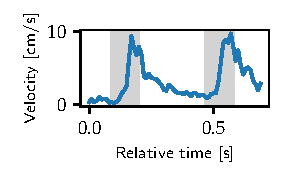
\includegraphics[scale=1]{smoothing}
\caption{Example result of the segmentation procedure.
  Shown is (non-smoothed) velocity.
  Areas shaded in gray were marked as acceleration, others as gliding.
\label{fig:smoothing}}
\end{marginfigure}
We then use the zero crossing of this smoothed acceleration to mark instances, where the fish moves from accelerating to gliding.
An example result for this method can be seen in figure~\ref{fig:smoothing}.
One acceleration and gliding phase is then combined to form a kick.
If an acceleration or gliding phase is shorter than a treshold \SI{0.08}{\s} the phase is merged with the previous one.
% kick_columns = [ 'fish_id', 'heading_change', 'heading_change_acc', 'duration', 'gliding_duration', 'length', 'max_vel', 'end_vel']
% social_columns = ['neighbor_distance', 'neighbor_angle', 'geometric_leader', 'viewing_angle_ltf', 'viewing_angle_ftl', 'rel_orientation',
%                     'x_f0', 'y_f0', 'x_f1', 'y_f1', 'angle_f0', 'angle_f1']
% wall_columns = [ f"wall_{type}{wall}_{id}" for id, type, wall in product( ['f0', 'f1'], ['distance', 'angle'],[0,1,2,3] )]

We then extract the heading change, length, maximum velocity for each kick.
Additionally, we extract the positions and angles of both fish and the distance and angles towards the wall for both fish for the kick and timesteps before it.
We include this data for the timesteps \(0, 5, \ldots, 35 \).

\subsection{Wall forces}
We begin with the modeling of wall-forces.
We follow a force-based modeling approach and describe the influence of a wall on the heading change \(\delta \phi_w\) as
\begin{equation*}
  \delta \phi_w (r_w, \theta_w) = f(r_w)O_w(\theta_w),
\end{equation*}
where $r_w$ corresponds to the distance to the wall and $\theta$ is the relative angle of the fish towars the wall~\autocite{calovi}.
We split the wall influence into an exponential decaying force term \(f_w\) and an odd angular-response function \(O_w\)
%todo: multiply by a constant
\begin{align*}
  f(r_w) &= \exp \left( -{(r_w/l_w)}^2 \right), \\
  O(\theta_w) &= \left(a_1 \sin(\theta_w) + a_2 \sin(2  \theta_w)  \right)  \left(1 +  b_1  \cos(\theta_w) + b_2 \cos(2  \theta_w) \right),
\end{align*}
where $l_w, a_1, a_2, b_1 \text{ and } b_2$ are parameters.
Note that we use a different series expansion for the odd angular function \(O_w\)%
\footnote{Their proposed form does not work in our case.
  The reason for this could be that they consider both a different species and a round wall.}.
Finally, we consider the closest two walls and sum over the influences
\begin{equation*}
 \delta \phi_w^{\text{total}} \left( \bm{r_w}, \bm{\theta_w} \right) = \sum_{i \in 2 \text{ closest walls}} \delta \phi_w^i (r_w^i, \theta_w^i).
\end{equation*}
The parameters are fit by minimizing the mean-squared error of heading change prediction using gradient-descent.
% todo: we do not actually use gradient descent but something different.

\subsection{Receptive Fields}
We now explain the input features of our social models.
From here on, we restrict our dataset to kicks where the wall influence is neglible.
Practically, we drop all kicks where the value of \(f_w(r_w)\) is larger than $0.1$.
Our social model use a receptive field as their input~\autocite{discreteModes}.
We construct this by rotating the coordinate system such that the fish we are considering is parallel to the x-axis and looking to the right.
This corresponds to a heading of \ang{0}.
We then shift the coordinate system such that our fish is at the center.

Or models then try to predict the product of a vector in direction of the heading change and the kick length.
This correspond to the kick trajectory in our new coordinate system.

We now shift our focus to the spatial discretization.
The standard approach is to divide the space into a regular grid of bins with equal size.
This approach has the disadvantage that some bins contain most of the kicks while others are nearly empty.
One solution to lessen the impact of this problem is to introduce a cut-off range, after which the social forces are assumed to be neglible.
We do not follow this approach but rather use a data-driven binning approach where we try to create bins that have a more balanced occupancy.
This is not the only criterion for choosing a discretization approach.
For interpratibility it is useful to be able to clearly distinguish situations where the other fish is behind or in front of the focal fish and whether it is on its left or right side.
We compare the occupancy of both the traditional and data-driven approach in figure xxx.
The algorithm to compute the bin edges is shown in algorithm~\ref{alg:binning}.
We only show how to compute the bins for the training set, the bins for the testing set can be computed in the same manner but without recomputing the edges.

\MakeRobust{\Call} % allow stacking of call
\begin{algorithm}[htb]
  \caption{%
\label{alg:binning}
    Data-driven Spatial Binning}

  \begin{algorithmic}
    \Ensure{\\$\textsc{Edges} (\bm{x}, N)$ computes the edges of a histogram s.t.\ all $N$ bins have the same number of elements.
      If this is not possible, the first few bins have a size that is 1 larger.\\
    $\textsc{Bin} (\text{edges}, \bm{x})$ computes the histogram bin from the bin edges with open boundaries on both sides.}
   \Function{Edges-1d}{$\bm{x}$}
    \Let{$\text{edges}^-$}{\Call{Edges}{$\bm{x} [\bm{x} \leq 0]$}}
    \Let{$\text{edges}^+$}{\Call{Edges}{$\bm{x} [\bm{x} > 0]$}}
    \State \Return \Call{Concatenate}{$\text{edges}^-, 0, \text{edges}^+$}
\EndFunction 
\Require{Positions of focal fish $(\bm{x}, \bm{y})$ an number of bins per axis $N$}
\Let{bins}{\Call{Array}{size = \Call{Len}{$\bm{x}$}}}
\Let{edges-x}{\Call{Edges-1d}{$\bm{x}$}}
  \Comment{First bin x-axis}
  \Let{bins-x}{\Call{Bin}{edges-x, $\bm{x}$}}
  \Let{edges-y}{\Call{Array}{$\text{size} = N$}}
  \For{$\text{bin-x} \in \text{bins-x}$}
  \Comment{Bin y-axis for each x-bin seperately}
  \Let{idx}{$(\text{bins-x} = \text{bin})$}
  \Let{$\bm{y}^{\text{cur}}$}{$\bm{y} [\text{idx}]$}
  \Let{$\text{edges-y}[\text{bin-x}]$}{\Call{Edges-1D}{$\bm{y}^{\text{cur}}$}}
  \Let{$\text{bins}[\text{idx}]$}{$\text{bin-x} \cdot N + \text{edges-y}[\text{bin-x}]$}
\EndFor
\Return{edges-x, edges-y, bins}
\end{algorithmic}
\end{algorithm}

This categorical feature bin is converted using one-hot-encoding to a feature vector.
We additionally use the standarized relative trajectory of the other fish multiplied with the aforementioned spatial feature%
\footnote{This can be generalized to multiple fish by interpreting the features as number of fish per bin and mean relative angle per bin.}.

\section{Social Models}\label{sec:social}
We are now ready to model the social behaviour of zebrafish.
Note that the approaches developed here can all be easily extended to larger fish groups.
Our target variable for all models is the relative kick trajectory in the local coordinate system described in the previous section.
We thus model heading change and distance jointly%
\footnote{This approach has two advantages.
  Firstly, we avoid dealing with cyclic data (as angles are).
Secondly, all target variables (i.e.\ vector components) have the same phsyical dimension and unit which makes the loss functions easier to interpret.}.
We start with a simple linear model.
This model is then refined twice by adding memory and non-linear effects.

\subsection{Linear receptive field model}
The linear model for a component \(i\) of our target vector \(\hat{\bm{y}}\) can be written as
\begin{equation*}
 \left( Y^i | \bm{\beta}^{i} \right)  \sim \mathcal{N} \left( \bm{X^i} \bm{\beta^i} + \text{ bias}, \sigma^2 \bm{I_{n \times p}}  \right),
\end{equation*}
where X is the design matrix.
In the following discussion we will drop the superscript for the component and describe the computation for one vector component without loss of generality.

\subsection{Time dependence}
We now add a time-dependence to our model.
To do this, we extract some time window before each kick.
For our experiments we use time steps of \SI{0}{\s}, \SI{0.05}{s}, \ldots, \SI{0.35}{\s}, which goes back roughly to the beginning of the last kick.

We consider two more models here.
For the first one we simply concatenate all features \(\beta_{i, t}\) for all timesteps \(t\).
This results in a very large number of parameters (\(\text{num. timesteps } \times \text{ num. bins}\)).

Alternatively, we can use the same spatial weights for each bin (i.e\ \( \forall t_1, t_2: \beta_{i, t_1} = \beta_{i, t_2}\)).
We then introduce a parameter \(c_t\) for each timestep and then use $c_t \beta_{i,t}$ as our parameters.
For consistency, we normalize all \(c_t\) such that they sum to unity.

\subsection{Mixture Density Networks: Bi-modal distributions \textit{\&} non-linearity}
As a final model we present a recurrent-neural network that predicts a full distribution for \(\left( \bm{y} | \bm{\beta} \right)\).
We start by describing an encoder, which transforms the input features to a hidden state, and a decoder which then transforms the hidden state into the output values.
The complete model is then an arbitrary combination of presented encoders and decoders.

We describe two simple encoders:
\begin{itemize}
\item The simplest (non-linear) choice is a multilayer-perceptron.
  In our case we use a two layers consisting of a linear transformation, followed by the \textit{tanh} non-linearity and a dropout\autocite{dropout} of 50\%.
  The input features for this model is the receptive field for the kick-off time.
\item
  As a temporal model we consider a standard recurrent neural network which has an input linear transformation, and a recurrent hidden-to-hidden connection.
  For the hidden-to-hidden connection we apply recurrent dropout.
  This means that we sample a dropout mask and apply this to the hidden-to-hidden connections for all sequence steps instead of sampling one per step.
  These two layers are added and transformed with a \textit{tanh} non-linearity
  \begin{equation*}
    \bm{h^i} (\bm{x}) = \operatorname{tanh} \left( \bm{w_{ih}} \bm{x^i} + \bm{w_{hh}} d (\bm{h^{i-1}}) \right),
  \end{equation*}
  where xxx.
  We learn the initial hidden state \(h^0\) instead of using a zero-initialised state.
  The input features for this models is the complete sequence of receptive fields leading to a kick.
  We use a fixed input sequence length for two reasons:
  Firstly, this allows us to compare linear models and \textsc{rnn}-models directly.
  Secondly, we avoid the assumption that a fish only considers its surroundings in the timespan between two kicks.
  \todo{Fix equation, add text}
\end{itemize}
Using more neurons in the hidden layer does not achieve better results here.
For scenarios with less sparse feature vectors such as with larger fish groups, a more complex representation might be beneficial.
We hope that the combination of the simplicity of the models coupled with the dropout regularization leads to a highly representative compressed representations in larger layers.
Note that both models (disregarding the learning initial \textsc{rnn}-state) have the same number of parameters.

We follow the basic idea of \textit{mixture density networks}\autocite{mdn} but use multivariate Gaussians with non-diagonal covariance as mixture components.
To do this, we write our prediction as
\begin{equation*}
p \left( \bm{y} | \bm{\beta} \right) = \sum_{i}^n \pi_i \mathcal{N} \left( \bm{\mu_i}, \bm{\Sigma_i} \right),
\end{equation*}
where \(\pi_i, \bm{\mu_i}, \bm{\Sigma_i}\) are the parameters for a mixture of Gaussians with \(k\) components and \(\mathcal{N}(\bm{\mu}, \bm{\Sigma_i})\) is a multivariate normal distribution 

These parameters are predicted for each target seperately by our neural network.
We will now derive necessary conditions that have to hold for the parameters and describe how our network output satisfies them.
Note that we can write the Cholesky decomposition
\footnote{This decomposition always exists for invertible covariance matrices as they are by definition positive-semidefinite and symmetric.}
of the covariance matrix \(\bm{\Sigma_i}\) as
\begin{equation*}
  \bm{\Sigma_i} = \bm{L_i} \bm{L_i^T} =
  \begin{bmatrix}
    a_i^2 & a_ib_i \\
    a_ib_i & b_i^2 + c_i^2
  \end{bmatrix} ,\quad
   \text{with } \bm{L} =
   \begin{bmatrix}
     a_i & 0 \\
     b_i & c_i
   \end{bmatrix}.
\end{equation*}
We then have to fulfil the following constraints:
\begin{itemize}
\item The diagonals of all \(\bm{L}_i\) need to be larger than zero.
  To do this we apply the \textit{softplus} non-linearity
  \begin{equation*}
   \operatorname{Softplus} (\bm{x}) = \log \left( 1 + \exp (\bm{x}) \right).
  \end{equation*}
  We add a small \(\varepsilon = 10^{-4}\) for numerical stability
  \footnote{This regularization reduces the condition number of \(\bm{\Sigma_i}\) by increasing the value of its minimal eigenvalue.
  Additionally it ensures that the variance has a minimal value and thus avoids degenerate distributions.}. % maybe cite this master's thesis?
  Using the fact that a matrix has an invertible Cholesky decomposition with positive diagonal elements iff.\ it is positive definite and Hermetian,
  the resulting matrix \(\bm{\Sigma_i}\) is a valid non-singular covariance matrix.
\item The mixing coefficients need to be positive and have to sum to one.
  This is achieved by using the \textit{softmax} non-linearity
  \begin{equation*}
    \operatorname{Softmax} (x_i) = \frac{\exp (x_i)}{\sum_j \exp (x_j)},
  \end{equation*}
  where \(x_i\) is one component of the output vector.
\end{itemize}
All other parameters can have arbitrary values.
We predict the Gaussian mixture parameters each by computing a linear transformation of the hidden state of the encoder followed by the appropiate non-linearity.


\section{Implementation \textit{\&} Training Details}
All neural networks were developed with PyTorch.
We use Adam with a learning rate of 0.01 and a weight decay of 0.001 to optimize our networks\autocite{adam}.
Encoders and decoders are jointly trained.

The linear model with identical spatial weights was also trained with PyTorch but with the \textsc{L-BGFS} optimizer.

The other linear models were trained with \textbf{scikit-learn}\autocite{scikitLearn}.
We used a grid search over the regularization parameters and chose the best w.r.t.\ the average cross-validation error.

\section{Evaluation}
% TODO: The following is not true!
%\marginnote{We can compare the log-likelihood of our models because they are \textit{nested} models, i.e.\ each model is a non-regularized \textsc{RNN} predicting parameters of mixtures of Gaussians with certain restrictions on the parameters.}
We start by comparing the angle prediction from the wall model.
Evaluating these prediction using the mean-squared-error (\textsc{mse}) or with similar metrics is not meaningful because they do not take the cyclical nature of angles into account.
For example, a prediction of \ang{159} for an angle of \ang{0} would be near-perfect but would incur a large \textsc{mse}-loss.
We rectify this by using results from directional statistics\autocite{circularStatistics}.
% Angle error, https://stats.stackexchange.com/questions/197639/calculating-goodness-of-fit-for-circular-data
We first define the mean angle as
\begin{equation*}
 \operatorname{Mean-Angle}(\bm{\alpha}) = \operatorname{arctan2} \left( \sum_i \sin \left( \alpha_i \right),  \sum_i \cos \left( \alpha_i \right)  \right).
\end{equation*}
One possible way of defining an error over angles is
\begin{equation*}
 \operatorname{Angle-Error}(\bm{\alpha}, \bm{\beta}) = \sum_i \operatorname{arccos} \left(  \cos  (\bm{\alpha} - \bm{\beta})  \right)_i.
\end{equation*}
This error is zero if both angles are identical.
Predicting the average angle leads to an error of xxx, using our model of xxx.
This error was estimated over the complete training and testing datasets.

We compare the models by the log-likelihood on the training and testing set.
As mentioned in chaper xxx, both datasets are restricted to situations with neglible wall-force.
This comparison captures the whole predictive distribution and not only the mean prediction.
In this way we take the uncertainty of the predictions into account.
Note that it is not straight-forward to use more complicated methods such as log-likelihood ratios or the Akaike information criterion because we cannot estimate the number of degrees of freedoms for penalized recurrent neural network models.

The results for the social models can be seen in table xxx.


\section{Conclusion \textit{\&} Future Work}
We presented different models for the behaviour of zebrafish.

Even though extending the models with a temporal and non-linear component did not show significant improvements, we think that the approaches are promising.
\begin{itemize}
\item The data-driven spatial discretization presented here results in a more equal distribution of fish.
\item Because the social models do not use properties of other animals directly but rather model the mean features per bin they extend trivially to larger animal groups, without changing the statistical models or the spatial discretization.
  This extension is harder for force-based models and usually require extensive modifications.
\item The explicit modelling of probability distributions allows us to sample from the trajectory distribution conditioned on the social surroundings and is able to predict bimodal distributions.
\end{itemize}

\printbibliography
\end{document}